\documentclass{article}
\usepackage[T1]{fontenc}
\usepackage{lmodern}
\usepackage{graphicx}
\usepackage{amsmath,amssymb}
\usepackage[a4paper,margin=2cm]{geometry}
\usepackage[absolute,overlay]{textpos}
\setlength{\TPHorizModule}{1mm}
\setlength{\TPVertModule}{1mm}
\usepackage[indonesian]{babel}
\usepackage{hyperref}
\setlength{\emergencystretch}{2em}
% unit: Halaman 47

\begin{document}

% === Halaman 47 (llm) ===

\vspace{103.95mm}

\section*{Kriptanalisis Vigenere Cipher}

\begin{itemize}
    \item Friedrich Kasiski adalah orang yang pertama kali memecahkan \textit{Vig\`enere cipher} pada Tahun 1863.
\end{itemize}

\vspace{10mm}

\begin{center}
\begin{tabular}{|l|}
\hline
\textcolor{red}{Friedrich Kasiski} \\
\textcolor{red}{Born: November 29, 1805 @} \textcolor{blue}{Schlochau, Kingdom of Prussia} \\
\textcolor{red}{Died: May 22, 1881 (aged 75) @} \textcolor{blue}{Neustettin, German Empire} \\
\textcolor{red}{Nationality:} \textcolor{blue}{German} \\
\hline
\end{tabular}
\end{center}

\vspace{5mm}

\begin{itemize}
    \item Metodenya dinamakan metode Kasiski
\end{itemize}

% deskripsi: Potret hitam putih Friedrich Kasiski
% bbox normalisasi: [0.8230, 0.0000, 0.9830, 0.3500]
\begin{textblock*}{33.60mm}(172.83mm,0.00mm)
\noindent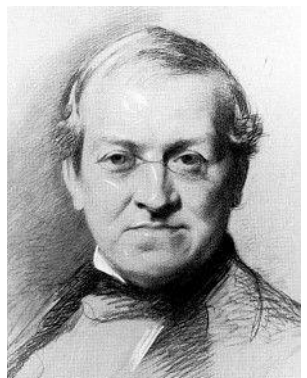
\includegraphics[width=33.60mm,height=103.95mm]{../../images/llm/page_047_img_01.png}%
\end{textblock*}

\end{document}
